%
% Documento: FRAMEWORK PROPOSTO
%
\chapter{ARQUITETURA DO PYBOT}\label{chap:imp}
    O \textit{framework} proposto foi formado por 4 módulos básicos, cada um com suas devidas utilidades e funções.
    A separação de cada módulo foi criada com base em suas características e funcionalidades, onde temos um modulo responsável pela gerenciamento e
    funcionamento do \textit{framework}, outro pela abstração das páginas dos sistemas \textit{web} a serem mapeados, controle e criação de relatórios
    e logs de execuções e por fim um responsável pelo download e gerenciamento dos \textit{drivers} de cada navegador utilizados pelos \textit{scripts}
    escritos pelos usuários.

    Na Figura \ref{fig:modules} é apresentado um diagrama dos módulos junto das suas classes principais que compõe o
    \textit{framework} e nas próximas seções serão descritas as suas funcionalidades e usos.


    \begin{figure}[H]
        \vspace*{0,3cm}
        \centering
        \caption{Diagrama de Componentes}
        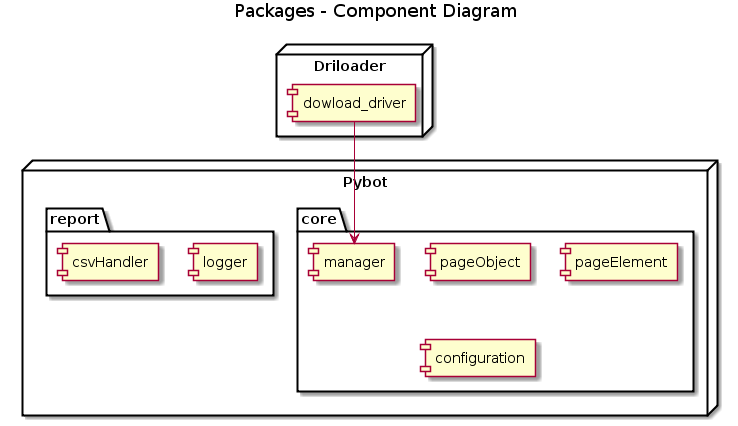
\includegraphics[width=1\textwidth]{./04-figuras/model}
        \label{fig:modules}
    \end{figure}

    \section{Core}
        Este é o módulo principal do framework, nele contém as funcionalidades básicas para a operação do \textit{framework} com o Selenium \textit{Webdriver},
        execução e o gerenciamento dos parâmetros de execuções de cada \textit{script}.

        \subsection{Manager} \label{sec:manager}
        A classe \textit{Manager} é a classe principal do framework, ela serve para abstrair o uso do Selenium \textit{Webdriver} criando uma camada
        de métodos próprios fazendo com que os \textit{scripts} criados com o \textit{Pybot} não sejam impactados por possíveis atualização na API do \textit{Selenium}.
        Dentro dele é feito o uso do \textit{Driloader}, descrito na subseção \ref{driloader} mais a frente, que verifica a necessidade do download do \textit{driver}
        para poder executar o \textit{Selenium Webdriver} e assim abrir o navegador escolhido pelo usuário.

        Como exemplo na Figura~\ref{fig:manager} temos o exemplo de alguns dos comandos disponíveis do Manager, sendo o da linha 4 para o início do processo
        e execução do \textit{driver} do navegador, na linha 7 para navegar para uma URL e na linha 12 para finalizar o processo.

        \begin{figure}[H]
            \vspace*{0,3cm}
            \centering
            \caption{Exemplo - Uso da classe Manager}
            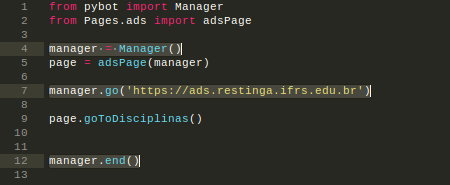
\includegraphics[width=0.8\textwidth]{./04-figuras/manager}
            \label{fig:manager}
        \end{figure}


        \subsection{Configuration}
        Responsável por gerar e gerenciar as configurações básicas para o \textit{framework} e disponibilizá-las no arquivo \textit{pybot.ini} diponivel na mesma pasta que
        o \textit{script}, caso não exista este arquivo é criado automaticamente para cada script. Nele é possível adicionar qualquer configuração ou parâmetros customizado
        do usuário para qualquer necessidade da execução do \textit{script}.

        Na Figura~\ref{fig:config} temos como exemplo apresentado na linha 8 é o código utilizado para buscar uma determinada configuração dentro arquivo \textit{pybot.ini}, sendo ela customizada pelo usuário ou não.

        \begin{figure}[H]
            \vspace*{0,3cm}
            \centering
            \caption{Exemplo - Uso do Configuration}
            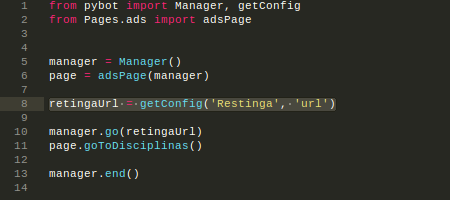
\includegraphics[width=0.8\textwidth]{./04-figuras/config}
            \label{fig:config}
        \end{figure}

        O padrão de escrita das configurações pode ser visto na \autoref{fig:pybot.ini}, onde é necessário ter uma Seção e as variáveis desejadas.
        E para a utilização delas segue o mesmo padrão: \\ \mbox{\textit{configuration.getConfig('Seção', 'variável')}}.

        \begin{figure}[H]
            \vspace*{0,3cm}
            \centering
            \caption{Estrutura pybot.ini}
            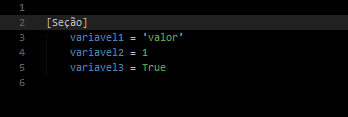
\includegraphics[width=0.7\textwidth]{./04-figuras/ini}
            \label{fig:pybot.ini}
        \end{figure}

        Para o funcionamento correto dos \textit{scripts} o \textit{Pybot} necessita de duas configurações básicas dentro desse arquivo, que são o navegador utilizado na execução e
        o endereço no computador do \textit{driver} desse navegador. Ambas configurações caso não existam são criadas automaticamente.



    \section{Component} \label{sec:comp}
        Módulo criado para seguir os padrões de \textit{PageObject} e \textit{PageElement}, contendo as classes de PageObject e PageElement e a classe responsável
        pela abstração para o \textit{WebElement} do \textit{Selenium Webdriver}.

        Pode-se observar na Figura \ref{fig:eleme} o uso das classes \textit{PageObject}, \textit{PageElement} e \textit{PageElements} nas linhas 3, 4 e 5 respectivamente.

        \begin{figure}[H]
            \vspace*{0,3cm}
            \centering
            \caption{Exemplo - Uso PageObject com PageElement e PageElements}
            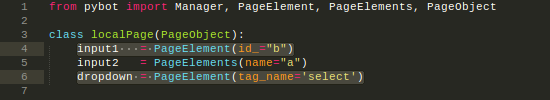
\includegraphics[width=1\textwidth]{./04-figuras/pageElement}
            \label{fig:eleme}
        \end{figure}

        \subsection{PageObject}
            Classe de abstração das páginas web. Serve para poder juntar diversos \textit{PageElement} descritos pelo usuário em uma classe para melhor legibilidade e componentização das
            páginas mapeadas e disponibilizar para os \textit{PageElement} acesso ao navegador.

        \subsection{WebElement}
            Serve para abstrair o uso da classe \textit{WebElement} do próprio \textit{Selenium Webdriver}. Contendo uma classe para cada tipo de campo dos \textit{html},
            ele dispõe de algumas funcionalidades básica, como a atribuição de um valor para um elemento do tipo \textit{input text} irá escrever
            valor dentro do campo, \textit{select} irá selecionar a opção cujo texto seja igual ao valor informado, \textit{radio} irá selecionar o
            a opção que tenha o \textit{value} do valor informado e para o tipo \textit{checkbox} irá marcar ou desmarcar as opções se o valor for
            verdadeiro (\textit{True}) ou falso (\textit{False})

        \subsection{PageElement e PageElements}
        \label{PageElement}
            Essas classes servem para controlar os elementos mapeados das telas. Sempre quando serão acessadas a classe faz novamente a pesquisa
            do elemento em tela, prevenindo assim uma das exceções mais comum do Selenium Webdriver que é a \textit{StaleElementReferenceException},
            que é quando o elemento em questão não existe mais no DOM ou a referência que tinha não é mais a mesma. Conta com uma lista de seletores
            que facilitam para o usuário buscar os elementos e deixam o código mais legível, os mesmos podem ser observados na Figura~\ref{fig:selectors}
            dentro de cada parênteses das definições dos \textit{PageElement}.
            Usa-se a classe PageElements quando quiser pegar mais de um elemento com o mesmo seletor.

            \begin{figure}[H]
                \vspace*{0,3cm}
                \centering
                \caption{Lista de Seletores}
                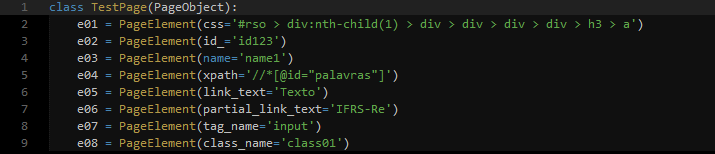
\includegraphics[width=1\textwidth]{./04-figuras/selectors}
                \label{fig:selectors}
            \end{figure}



    \section{Report}

        Este módulo é destinado para geração de \textit{logs} das execuções internas do \textit{framework}, a criação e controle
        de \textit{logs} de execuções de texto e no terminal definidos pelos usuário e a criação de planilhas analíticas de dados extraídos das páginas.

        \subsection{Logger}
        Classe de geração dos \textit{Logs} de execução do \textit{framework}, onde cada execução, ação, sucessos e falhas podem ser configurados para que no
        decorrer do processo sejam mostrados no terminal de execução e no final salvos em um arquivo de texto.

        Os \textit{logs} podem ser configurados com níveis que podem ser \textit{CRITICAL}, \textit{ERROR}, \textit{WARNING}, \textit{INFO} e \textit{DEBUG}, e no arquivo de configurações
        é possível definir qual o nível desejado para que os \textit{logs} apareçam. Numa escala de 1 a 5, \textit{CRITICAL} tem valor 5 e \textit{DEBUG} valor 1, dessa maneira se o nível
        do \textit{log} for definido como \textit{DEBUG} apenas ele aparecerá e se for definido como \textit{CRITICAL} todos apareceram.

        Na \autoref{fig:logs} podemos verificar 2 tipos de escritas do \textit{log}, onde na linha 11 temos a escrita de um \textit{log} e na linha 21 é o tratamento
        de erros de execução, onde este para a execução do código ao ser chamado.

        \begin{figure}[H]
            \vspace*{0,3cm}
            \centering
            \caption{Exemplo - Uso do Logger}
            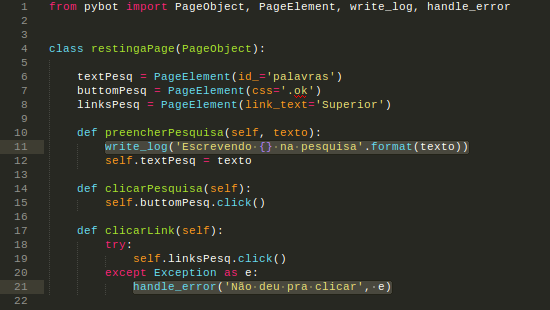
\includegraphics[width=0.9\textwidth]{./04-figuras/logs}
            \label{fig:logs}
        \end{figure}


        \subsection{CsvHandler}
        Utilizado para geração de planilhas com dados extraídos das páginas para análise posterior dos usuários. Os dados têm que ser extraídos manualmente pelo
        usuário, e uma vez extraídos são salvos automaticamente em um arquivo com a extensão \textit{csv}.

        Como exemplo, podemos observar na \autoref{fig:csv} um exemplo de utilização do \textit{CsvHandler}, onde, na linha 5 será criado uma planilha contendo uma
        coluna Disciplina e na linha 21 será inserido registros na planilha abaixo da coluna.

        \begin{figure}[H]
            \vspace*{0,3cm}
            \centering
            \caption{Exemplo - Uso do CsvHandler}
            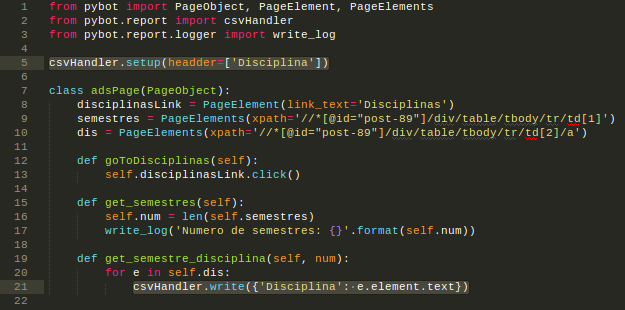
\includegraphics[width=0.9\textwidth]{./04-figuras/csv}
            \label{fig:csv}
        \end{figure}


    \section{Driloader}
    \label{driloader}
        Driloader é o responsável pelo download dos \textit{drivers} de cada navegador, suportando \textit{download} dos \textit{drivers} do \textit{Internet Explorer},
        \textit{Firefox} e \textit{Chrome}, sendo possível para o usuário selecionar uma versão específica, a última versão ou detectar automaticamente qual a versão adequada para o navegador
        instalado do usuário. Como para utilização do \textit{Selenium Webdriver} é necessário um \textit{driver} específico de cada navegador foi tomada a decisão da criação
        desse projeto que inicialmente era um módulo do \textit{framework}, mas pela autonomia e praticidade que ele proporciona aos usuários do Selenium Webdriver foi feita a
        separação dele do \textit{Pybot}. Seu uso é feito na classe Manager (\autoref{sec:manager}) automaticamente quando nenhuma \textit{driver} é encontrado no computador do usuário.



